\documentclass[12,]{article}
\usepackage{lmodern}
\usepackage{amssymb,amsmath}
\usepackage{ifxetex,ifluatex}
\usepackage{fixltx2e} % provides \textsubscript
\ifnum 0\ifxetex 1\fi\ifluatex 1\fi=0 % if pdftex
  \usepackage[T1]{fontenc}
  \usepackage[utf8]{inputenc}
\else % if luatex or xelatex
  \ifxetex
    \usepackage{mathspec}
    \usepackage{xltxtra,xunicode}
  \else
    \usepackage{fontspec}
  \fi
  \defaultfontfeatures{Mapping=tex-text,Scale=MatchLowercase}
  \newcommand{\euro}{€}
\fi
% use upquote if available, for straight quotes in verbatim environments
\IfFileExists{upquote.sty}{\usepackage{upquote}}{}
% use microtype if available
\IfFileExists{microtype.sty}{%
\usepackage{microtype}
\UseMicrotypeSet[protrusion]{basicmath} % disable protrusion for tt fonts
}{}
\usepackage[margin=1in]{geometry}
\usepackage{graphicx}
\makeatletter
\def\maxwidth{\ifdim\Gin@nat@width>\linewidth\linewidth\else\Gin@nat@width\fi}
\def\maxheight{\ifdim\Gin@nat@height>\textheight\textheight\else\Gin@nat@height\fi}
\makeatother
% Scale images if necessary, so that they will not overflow the page
% margins by default, and it is still possible to overwrite the defaults
% using explicit options in \includegraphics[width, height, ...]{}
\setkeys{Gin}{width=\maxwidth,height=\maxheight,keepaspectratio}
\ifxetex
  \usepackage[setpagesize=false, % page size defined by xetex
              unicode=false, % unicode breaks when used with xetex
              xetex]{hyperref}
\else
  \usepackage[unicode=true]{hyperref}
\fi
\hypersetup{breaklinks=true,
            bookmarks=true,
            pdfauthor={Instituto Tecnológico Autónomo de México; Edwin Cházaro Argueta cu 153848; Andrea Fernández Conde cu 104499; Andrea García Tapia cu 104050},
            pdftitle={Estadística Espacial: Tarea 2},
            colorlinks=true,
            citecolor=blue,
            urlcolor=blue,
            linkcolor=magenta,
            pdfborder={0 0 0}}
\urlstyle{same}  % don't use monospace font for urls
\setlength{\parindent}{0pt}
\setlength{\parskip}{6pt plus 2pt minus 1pt}
\setlength{\emergencystretch}{3em}  % prevent overfull lines
\setcounter{secnumdepth}{5}

%%% Use protect on footnotes to avoid problems with footnotes in titles
\let\rmarkdownfootnote\footnote%
\def\footnote{\protect\rmarkdownfootnote}

%%% Change title format to be more compact
\usepackage{titling}
\setlength{\droptitle}{-2em}
  \title{Estadística Espacial: Tarea 2}
  \pretitle{\vspace{\droptitle}\centering\huge}
  \posttitle{\par}
  \author{Instituto Tecnológico Autónomo de México \\ Edwin Cházaro Argueta cu 153848 \\ Andrea Fernández Conde cu 104499 \\ Andrea García Tapia cu 104050}
  \preauthor{\centering\large\emph}
  \postauthor{\par}
  \predate{\centering\large\emph}
  \postdate{\par}
  \date{29 de abril de 2015}


\usepackage{float}
\usepackage{morefloats}
\usepackage[spanish]{babel}
\usepackage{graphicx}
\usepackage{tcolorbox}
\usepackage{rotating}
\usepackage{longtable}
\usepackage{colortbl}
%\usepackage{natbib}
%\newenvironment{scaleb}{ \scalebox{0.4}{} {} }
%\newenvironment{scaleb}{ \tiny{} }
% biber
\usepackage[autostyle]{csquotes}

\usepackage[
    backend=biber,
    style=authoryear-icomp,
    sortlocale=de_DE,
    natbib=true,
    url=false,
    doi=true,
    eprint=false
]{biblatex}
\addbibresource{bibliografia.bib}

\usepackage[]{hyperref}
\hypersetup{
% Turn on this if you prefer to have links colored instead of marked with squares
colorlinks = true,
linkcolor = black,
urlcolor = blue,
citecolor = black,
% pdfpagemode = UseNone
}

\renewcommand\figurename{Figura}
\renewcommand\tablename{Tabla}

\newenvironment{myexampleblock}[1]{%
    \tcolorbox[beamer,%
    noparskip,breakable,
    colback=LightGreen,colframe=DarkGreen,%
    colbacklower=LimeGreen!75!LightGreen,%
    title=#1]}%
    {\endtcolorbox}

\newenvironment{myalertblock}[1]{%
    \tcolorbox[beamer,%
    noparskip,breakable,
    colback=LightCoral,colframe=DarkRed,%
    colbacklower=Tomato!75!LightCoral,%
    title=#1]}%
    {\endtcolorbox}

\newenvironment{myblock}[1]{%
    \tcolorbox[beamer,%
    noparskip,breakable,
    colback=LightBlue,colframe=DarkBlue,%
    colbacklower=DarkBlue!75!LightBlue,%
    title=#1]}%
    {\endtcolorbox}


\begin{document}

\maketitle


{
\hypersetup{linkcolor=black}
\setcounter{tocdepth}{2}
\tableofcontents
}
\pagebreak

\section{Introducción}\label{introduccion}

Las montañas Azules (en inglés, \emph{Blue Mountains}) son una cadena
montañosa localizada en el noroeste de los Estados Unidos, que se
extiende largamente por el este del estado de Oregón y el sudeste de
Washington. Tiene una superficie muy accidentada y seca de 10,500 km²
que se extiende desde el este y sureste de Pendelton, Oregon hasta el
rio Snake con la frontera de Idaho.

\begin{figure}[H]
\centering
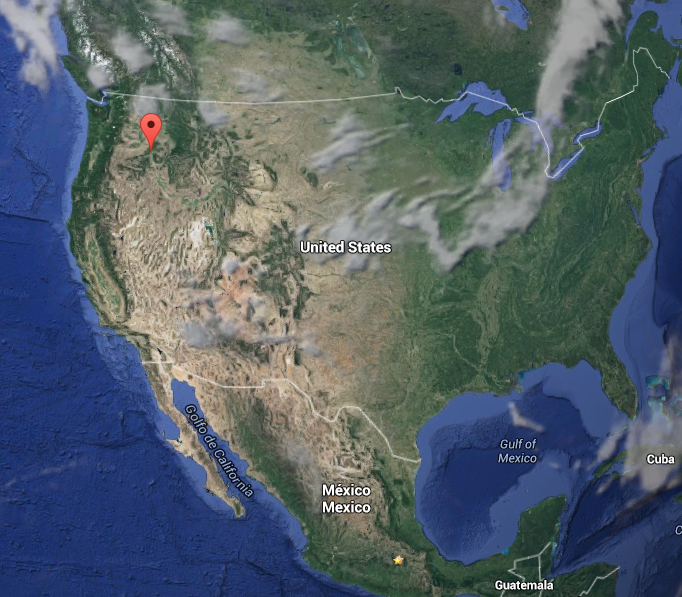
\includegraphics[width=0.55\textwidth]{imagenes/usa.png}
\caption{Ubicación geográfica de las montañas azules.}

\end{figure}

Las Montañas Azules contienen 3 parques nacionales y varias áreas
naturales protegidas tales como el Malheur National Forest, Umatilla
National Forest, Wallowa-Whitman National Forest, Umatilla Wilderness,
North Fork John Day Wilderness, Strawberry Mountain Wilderness y la
Monument Rock Wilderness\footnote{Blue Mountains
  \url{http://geonames.usgs.gov/apex/f?p=gnispq:3:0::NO::P3_FID:1154280}.}.

Dada su geografía y vegetación la zona de las Montañas Azules es
propensa a incendios. La información que comprende este estudio
corresponde a incendios que comenzaron entre el 01 de abril de 1986 al
31 de julio de 1993 en los 3 estados que abarca la zona de las Montañas
Azules (Oregon, Washington e Idaho).

\begin{figure}[H]
\centering
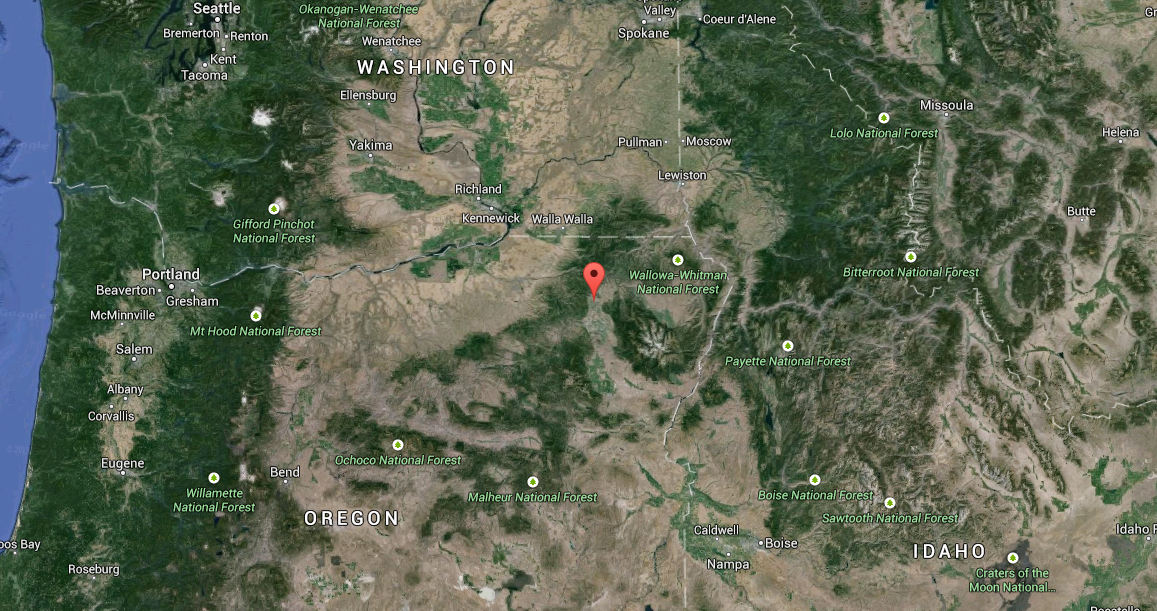
\includegraphics[width=0.6\textwidth]{imagenes/blueM.png}
\caption{Parques nacionales de la zona.}

\end{figure}

\section{Descripción del Área de
Estudio}\label{descripcion-del-area-de-estudio}

Se cuenta con tres fuentes de datos: información de incendios,
información geográfica y los polígonos que definen el área.

De 5778 incendios en la zona se cuenta con la coordenada geográfica, la
fecha (día, mes y año), tamaño, elevación, pendiente, orientación de la
ladera donde ocurrió el incendio (\emph{aspect}) y vegetación
(\emph{veg9}). A partir de esas variables se genera la variable de
estación (\emph{estac}) considerando como puntos de corte para los
mismos el 21 de marzo, 21 de junio, 21 de septiembre y 21 de diciembre.
Asimismo, se categorizan las variables de elevación y orientación de la
ladera con 6 cortes equidistantes en el rango de su dominio. Los datos
modificados se ejemplifican en el Cuadro 1.

Toda la región se caracteriza en la información geográfica y poligonal
adicional. En la primera se incluyen coordenadas (latitud, longitud y
elevación), orientación de la ladera, pendiente y vegetación en 8089
puntos. En la segunda se definen polígonos a partir de 2130 coordenadas.

\begin{table}[H]
\centering
{\tiny
\begin{tabular}{rrrrrrrrrrrlllll}
  \hline
lon & lat & yr & mo & day & size & elev & slope & aspect & dia & veg9 & mo2 & day2 & estac & elev\_cat & aspect\_cat \\
  \hline
764.49 & 816.11 &  86 &   4 &  14 & 0.10 & 1463 &   2 & 302.00 &  13 &   1 & 04 & 14 & Primavera & (1.15e+03,1.53e+03] & oeste \\
  569.35 & 747.68 &  86 &   5 &  20 & 0.20 & 1310 &   3 & 26.00 &  49 &   5 & 05 & 20 & Primavera & (1.15e+03,1.53e+03] & norte \\
  542.17 & 700.37 &  86 &   5 &  26 & 0.10 & 1707 &   2 & 168.00 &  55 &   6 & 05 & 26 & Primavera & (1.53e+03,1.92e+03] & sur \\
  640.66 & 753.46 &  86 &   5 &  28 & 5.00 & 1400 &   8 & 228.00 &  57 &   5 & 05 & 28 & Primavera & (1.15e+03,1.53e+03] & oeste \\
  510.35 & 646.56 &  86 &   5 &  29 & 11.00 & 1405 &   2 & 43.00 &  58 &   8 & 05 & 29 & Primavera & (1.15e+03,1.53e+03] & norte \\
  538.01 & 741.06 &  86 &   5 &  30 & 0.10 & 1404 &   2 & 252.00 &  59 &   1 & 05 & 30 & Primavera & (1.15e+03,1.53e+03] & oeste \\
   \hline
\end{tabular}
}
\caption{Muestra de los datos a utilizar.}
\end{table}

Para determinar las relaciones existentes entre las características
geográficas y la ocurrencia de incendios, se realizaron una serie de
exploraciones gráficas. En la Figura \ref{mapaincendios} se superponen
los incendios (amarillo) en el terreno coloreado por altitud (se
establece un rango de colores en el que el mínimo es verde claro y el
máximo es café). El tamaño de los círculos amarillos refiere a la
extensión del mismo.

\begin{figure}[H]
\centering
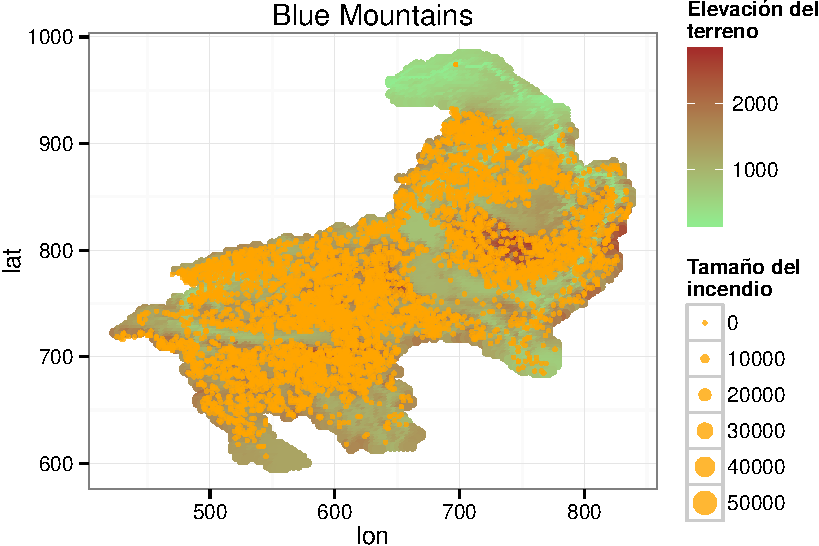
\includegraphics{tarea2_files/figure-latex/mapaincendios-1.pdf}
\caption{Mapa de elevación y tamaño de incendios de la zona.}
\label{mapaincendios}
\end{figure}

A partir de la Figura \ref{mapaincendios} se observa un indicativo claro
de la existencia de una relación importante entre los incendios y la
altitud. Aunque las únicas áreas libres de amarillo (incendios) son las
de altitud baja, no es claro que los incendios se concentren en las
zonas de mayor altitud. Al contrario, parece haber un rango de elevación
a la baja y a la alta que inhibe la existencia de incendios. Al revisar
los mapas anuales en la figura \ref{mapaincendiosanio}, se observa que
se mantiene la relación entre la elevación y el tamaño de los incendios.

\begin{figure}[H]
\centering
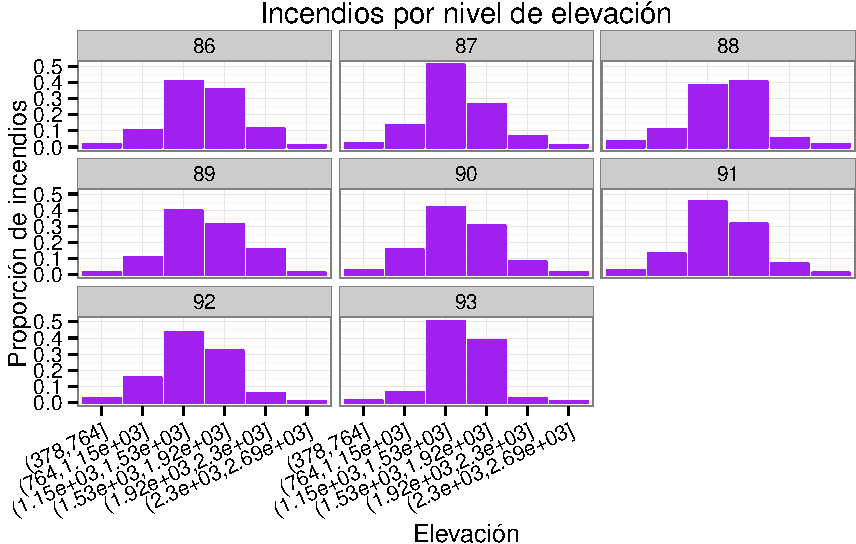
\includegraphics[width=0.7\textwidth]{tarea2_files/figure-latex/unnamed-chunk-3-1.pdf}
\caption{Mapa del tamaño de incendios por terreno y año.}
\label{mapaincendiosanio}
\end{figure}

\begin{figure}[H]
\centering
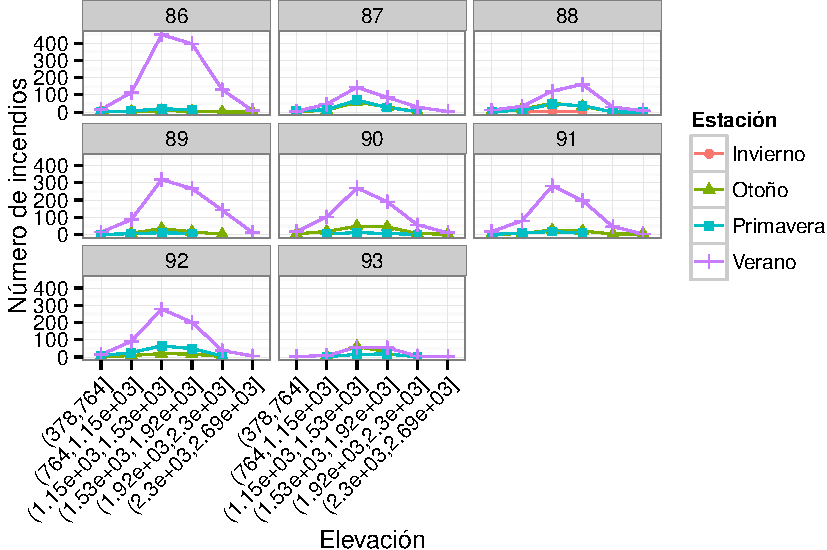
\includegraphics[width=0.7\textwidth]{tarea2_files/figure-latex/unnamed-chunk-4-1.pdf}
\caption{Proporción de incendios por nivel de elevación y año.}
\label{barraincendios}
\end{figure}

Para clarificar la relación entre estas dos variables, se grafica por
año la elevación categorizada contra la proporción de incendios. En la
Figura \ref{barraincendios} se observa que la mayoría de los incendios
se concentran en un rango de elevación de entre 1150 a 1920 (categorías
3 y 4 en la variable generada). Para otras altitudes, la cantidad de
incendios es mucho menor. Al refinar la relación e introduciendo la
estación, se observa que ésta se mantiene para las distintas estaciones.
En la Figura \ref{estelev} se gráfica a la variable categórica de
elevación contra el número de incendios por estación y segmentado por
año.

\begin{figure}[H]
\centering
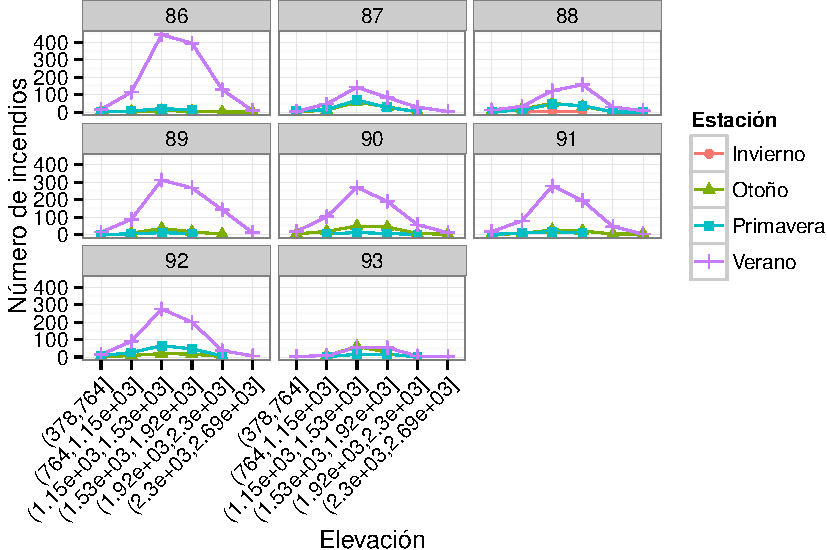
\includegraphics{tarea2_files/figure-latex/unnamed-chunk-5-1.pdf}
\caption{Número de incendios por elevación, año y estación.}
\label{estelev}
\end{figure}

Lo primero que se rescata de la Figura \ref{estelev} es que en el
invierno la cantidad de incendios es muy limitada y en el verano es
considerablemente mayor que en el resto de las estaciones. Esto tiene
que ver con las variaciones de temperatura a lo largo del año. Ahora
bien, la asociación entre las categorías 3 y 4 de elevación y la
cantidad de incendios se mantiene con algunas variaciones entre años.
Para entender mejor la asociación observada, se estudia más a detalle
las posibles causas de esta relación.

Los incendios están asociados al tipo de vegetación y por ende a la
altitud, fenómenos meteorológicos como las sequías también son un factor
que favorecen los incendios. Existen diferentes maneras de medir la
severidad de las sequías, para este estudio utilizamos el Índice de
Severidad de Sequía de Palmer (PDSI) que mide el nivel de sequía a
partir de la precipitación y temperatura reciente.

En la figura 5 se puede observar que en primavera de 1987, invierno de
1988 y verano de 1989 hubo mayores incendios. Si observamos el Índice de
Palmer de la estación anterior a esas temporadas nos damos cuenta que
hubo sequías severas en la zona de las Montañas Azules.

\begin{figure}[H]
\centering
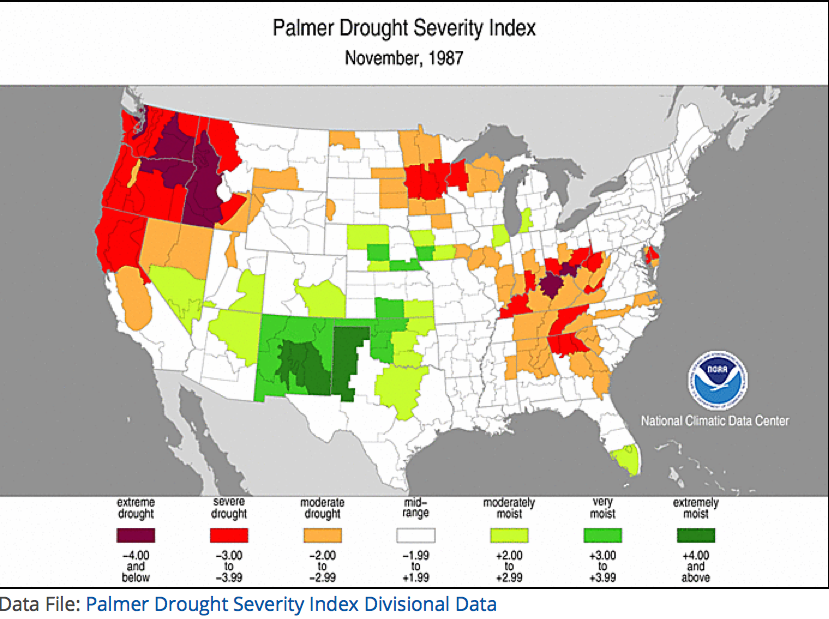
\includegraphics[width=0.5\textwidth]{imagenes/IP87.png}
\caption{Índice de Palmer de severidad en sequías, 1987\footnote{\url{http://www.ncdc.noaa.gov/temp-and-precip/drought/historical-palmers/psi/198304-199307}}.}

\end{figure}

\begin{figure}[H]
\centering
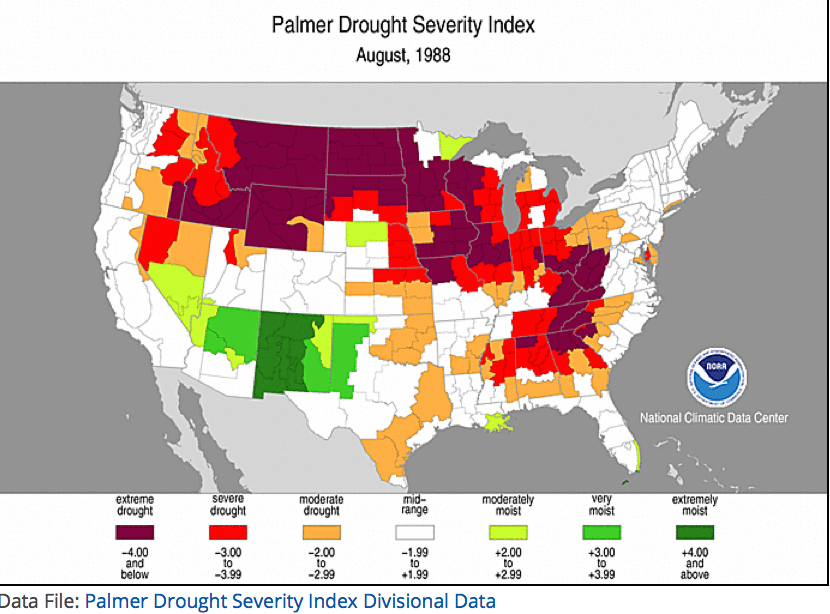
\includegraphics[width=0.5\textwidth]{imagenes/IP88.png}
\caption{Índice de Palmer de severidad en sequías, 1988.}

\end{figure}

\begin{figure}[H]
\centering
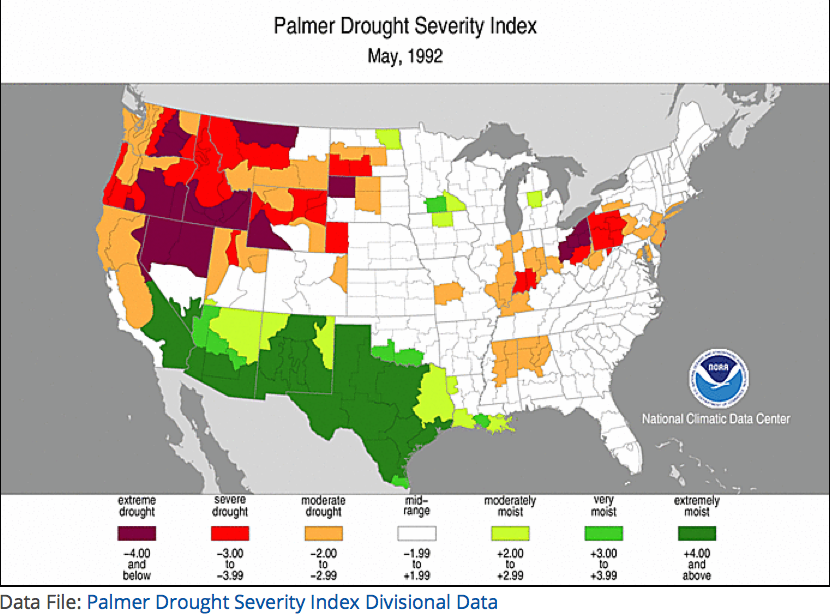
\includegraphics[width=0.5\textwidth]{imagenes/IP92.png}
\caption{Índice de Palmer de severidad en sequías, 1989.}

\end{figure}

Podemos observar que en verano y primavera ocurren más incendios, y en
el 4 y 5 corte de elevación. Si lo analizamos por año\footnote{\url{http://www.ncdc.noaa.gov/temp-and-precip/drought/historical-palmers/phd/198304-199307}}
en 1986 hubo más incendios en verano, esto se debe a que en ese año hubo
fenómeno de \emph{El Niño} de julio de 1886 a marzo de 1988\footnote{\url{http://www.cpc.ncep.noaa.gov/products/analysis_monitoring/ensostuff/ensoyears.shtml}}.
El fenómeno de ``El Niño'' es una oscilación del sistema
océano-atmósfera en el Pacífico tropical que tiene consecuencias
importantes para el clima en todo el mundo\footnote{\url{http://www.pmel.noaa.gov/tao/elnino/el-nino-story.html}}
mientras que en lugares cercanos al trópico genera tormetas tropicales,
en el norte genera sequías.

Ahora, el objetivo es explorar la composición de la vegetación según
elevación y la proporción de incendios. En la figura \ref{vegetacion} se
exhiben, para diferentes niveles de elevación, las proporciones de
incendios coloreadas por el tipo de vegetación. Recordemos que las
elevaciones con mayor número de incendios eran la 3 y la 4. Este
gráfico, aunado a lo observado anteriormente, nos permite distinguir que
son las vegetaciones 6, 7 y 8 las que caracterizan a las elevaciones 3 y
4 en cuanto a la proporción de incendios. Las demás categorías de
asociación tienen asociadas otras vegetaciones con mayor proporción de
incendios.

\begin{figure}[H]
\centering
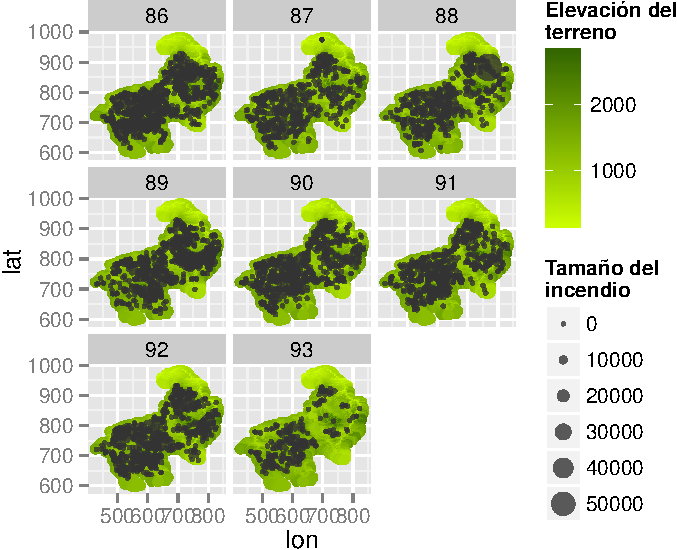
\includegraphics{tarea2_files/figure-latex/unnamed-chunk-6-1.pdf}
\caption{Incendios por elevación, tipo de vegetación y estación.}
\label{vegetacion}
\end{figure}

Ahora bien, buscamos entender la relación que existe entre la vegetación
y los incendios. Para esto, en la figura \ref{elevveg} se muestra un
gráfico de barras para cada categoría de elevación con el número de
incendios por cada tipo de vegetación. Los tipos de vegetación más
propensos a incendios son el 5, 6 y 7.

\begin{figure}[H]
\centering
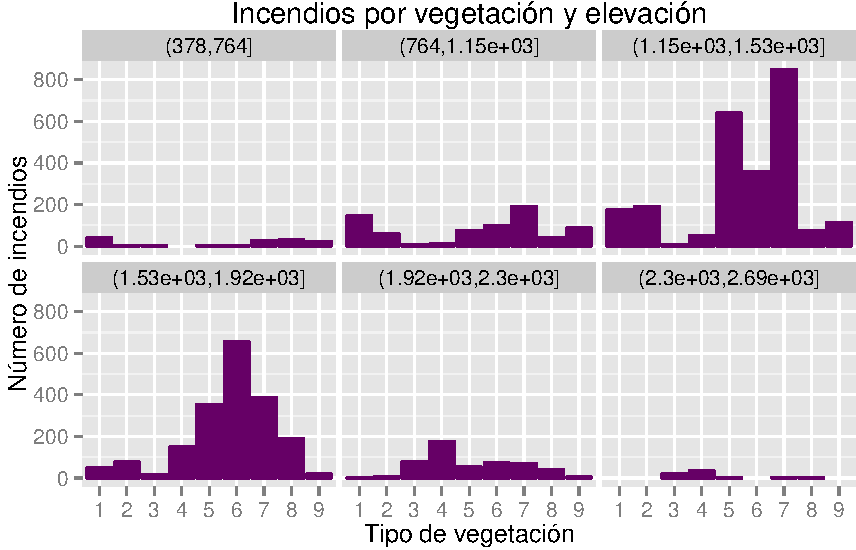
\includegraphics[width=0.7\textwidth]{tarea2_files/figure-latex/unnamed-chunk-7-1.pdf}
\caption{Incendios por elevación, vegetación y estación.}
\label{elevveg}
\end{figure}

En cuanto a la variable de \emph{aspect} u orientación de la ladera
donde ocurrió el incendio, se utilizó la variable recategorizada para
explorar las relaciones con el número de incendios y el tamaño de los
mismos. Sin embargo, ninguna de los análisis realizados mostró alguna
relación importante entre éstas. Por ende, no se incluye esta variable
en los modelos realizados. Contra el tamaño de incendios, se probó la
media y la mediana sin ninguna diferencia. En la siguiente figura, se
muestra el número de incendios según la orientación de la ladera para
cada año. Sin embargo, en este caso tampoco hay relación.

\begin{figure}[H]
\centering
\includegraphics[width=0.7\textwidth]{tarea2_files/figure-latex/unnamed-chunk-8-1.pdf}
\caption{Número de incendios por orientación de la ladera por año.}
\end{figure}

\section[Metodología]{Metodología\footnote{Esta sección se basó en las
  notas de clase ``Procesos Puntuales'' impartidas por el Dr.~Carlos
  Díaz}}\label{metodologia}

En los procesos puntuales nos interesa saber si el conjunto de puntos
distribuidos en una área fija fue generado por un proceso estocástico.
Existen tres tipos de patrones: \emph{regulares, aleatorios o clusters}.
Para poder determinar qué tipo de patrón siguen es necesario hacer
pruebas de Aleatoriedad Espacial Completa (AEC o \emph{CSR en inglés}).

La AEC se puede definir como un proceso Poisson homogéneo (PPH) en
$\mathbb{R}^n$, esto es, el número de puntos contenidos en cualquier
región $A$, $N(A)$, sigue una distribución Poisson con media
$\lambda \vert A \vert$; donde $\vert A \vert$ es el área de la región
$A$ y $\lambda$ es el parámetro de intensidad del proceso y además los
puntos en la región $A$ se distribuyen de manera aleatoria e
independiente con distribución uniforme en $A$. Esto significa que si
esta hipótesis fuera cierta, entonces los eventos (incendios en este
caso) ocurren totalmente al azar, de forma constante en la región y que
no hay interacción entre eventos.

Existen dos tres tipos de estadísticos: los basados en conteos, los
basados en proximidad con el vecino y los basados en propiedades de la
función de intensidad (primer y segundo orden). El primer estadístico es
el filtro para definir si existe AEC, si se rechaza la hipótesis de AEC
se utilizan los otros dos para poder definir si es un patrón regular o
un patron agregado (cluster)

\subsection{Estadísticos Basados en
Conteos}\label{estadisticos-basados-en-conteos}

Entre los estadísticos usados para probar AEC están los basados en
conteos. Suponemos una partición de la región de interés $A$ en $m$
cuadrantes y en cada uno hay $n_1, n_2, ..., n_m$ eventos. El
estadístico más básico es la \textit{Razón Varianza Media} (VMR en
inglés) \[
VMR = \frac{Varianza(y)}{Media(y)}, y = N
\]

Si $VMR < 1$ indica uniformidad en los eventos o puntos, $VAR(Y) = 0$
perfectamente uniforme , $VMR > 1$ indica culster y si $VMR = 1$ indica
aleatoriedad.

Exite otra medida basada en conteos llamada \emph{índice de dispersión},
el índice se define como\\\[
I = \sum\limits_{i=1}^m \dfrac{(n_i - \overline{n})^2}{(m-1) \overline{n}}
\] que bajo AEC debe tomar valor igual a $1$.

Otro estadístico que se usa es \[
I' =  \dfrac{(m-1)\sum\limits_{i=1}^m (c_i - \overline{c})^2}{\overline{c}} = (m-1)I
\]

Bajo AEC $I' \sim \chi^2_{(m-1)}$, por lo que se rechaza la hipótesis de
AEC al nivel de significancia $\alpha$ si
$I' > \chi^2_{(m-1)(1 - \alpha)}$.

\subsection{Estadísticos Basados en Distancias al Vecino
Próximo}\label{estadisticos-basados-en-distancias-al-vecino-proximo}

También existen otros basados en distancias entre puntos o eventos, uno
de ellos es el vecino más cercano, ya sea desde un punto $x$ del patrón
observado, o desde un punto arbitrario.

Por último la $K$ de Ripley, se define como\footnote{\# extra de eventos
  dentro de una distancia $h$ a un evento arbitrario} \[
K(h) = \dfrac{1}{\lambda} \mathbb{E}.
\]

Para el caso del método basado en distancias se define la variable
aleatoria $D$ como la distancia de un evento arbitrario al evento más
cercano, entonces, bajo AEC,

\[
\mathbb{P}(D>d) = 1 - e^{- \lambda \pi d^2}.
\]

Entonces la media y la varianza de $D$ son
$\mathbb{E}[D] = \dfrac{1}{2 \sqrt{\lambda}}$ y
$Var[D] = \dfrac{4 - \pi}{4 \lambda \pi}$. Por esto, si se defina
$\overline{D}$ como la media muestral de las distancias, asumiendo $n$
v.a.i.i.d., se tiene que
$\mathbb{E}[\overline{D}] = \dfrac{1}{2 \sqrt{\lambda}}$ y
$Var[\overline{D}] = \dfrac{4 - \pi}{4 n \lambda \pi}$; por lo que
centrando

\[
Z = \dfrac{\overline{D} - 1/ (2 \sqrt{\lambda})}{\sqrt{(4-\pi)/(4n\pi\lambda)}} \underset{n \to \infty}{\sim} N(0,1).
\]

Así, si $n$ es grande, el IC para AEC tendrá la forma
$\overline{D} \pm Z_{1- \alpha / 2} \sqrt{(4-\pi)(4n\pi\lambda)}$.

En el caso de la $K$ de Ripley, si hubiera AEC entonces
$K(h) = \pi h^2$, pues el número de puntos dentro de un radio $h$ debe
ser proporcional al área del círculo de radio $h$. Si los datos
estuvieran en conglomerados, uno esperaría que $K(h) > \pi h^2$,
mientras que si hubiera algún tipo de repulsión se esperaría que
$K(h) < \pi h^2$. La versión muestral de la $K$ de Ripley es \[
\hat{K}(h) = \dfrac{\vert A \vert}{n^2} \sum\limits_{i=1}^{n} \sum\limits_{i \neq j}^{} \dfrac{I_h(d_{ij})}{w_{ij}}
\] donde $m$ es el número de eventos en $A$, $w_{ij}$ es la proporción
del círculo con centro en $i$ y que pasa por $j$ que está dentro de $A$,
$d_{ij}$ es la distancia entre los puntos $i$ y $j$, $I$ es la función
indicadora para la distancia $d_{ij}$.

Muchas veces se usa la función $L(h) = \sqrt{\dfrac{K(h)}{\pi}} - h$,
pues la varianza de $L$ es aproximadamente constante bajo AEC. En la
práctica se grafica $t - \hat{L}(t)$ contra $t$, la cual, en el caso de
AEC, deberá ser aproximadamente una línea horizontal en el cero.

Si se rechaza la hipótesis de AEC, se deben considerar procesos no
homogéneos. La extensión más simple es el Proceso Poisson no homogéneo
(PPNH), el cual cumple los mismos principios de el PPH, excepto que la
función de intensidad depende del sitio, $\lambda(x)$. Entonces, para un
área $B \subset A$, se tiene que \[
\mathbb{E}[N(B)] = \int_{B} \lambda(u) du
\]

y

\[
\mathbb{P}(N(b) = n) = \dfrac{[\int_{B} \lambda(u) du]^n \exp^{\int_{B} \lambda(u) du}}{n!}
\]

A este modelo se le pueden agregar más covariables referentes al sitio;
por ejemplo, la elevación y la humedad del sitio.

\subsection{Función de Intensidad (primer y segundo
orden)}\label{funcion-de-intensidad-primer-y-segundo-orden}

Tomado \emph{dx} como una pequeña región que contiene el punto x la
función de intensidad de \textbf{primer orden} es

\[
\lambda(x) = \displaystyle\lim_{dx \rightarrow 0} \dfrac{E[N(dx)]} {\textbar{dx}\textbar}
\]

y la de \textbf{segundo orden} es \[
\lambda_2(x,y) = \displaystyle\lim_{dx, dy \rightarrow 0} \dfrac{E[N(dx)N(dy)]} {\textbar{dx}\textbar \textbar{dy}\textbar}
\]

La intensidad de primer orden $\lambda$ se interpreta como el número
esperado de eventos por unidad de área mientras que la segunda tiene una
interpretación más complicada. Hay dos maneras de estimarla : métodos no
paramétricos y métodos paraétricos, En el primero no hay ningun modelo
involucrado y por lo general se usasn conteos de cuadrantes o estimación
por kernel. Los segundos utilizan un modelo paramétrico y de utiliza la
Máxima Verosimilitud o Máxima Pseudoverosimilitud.

\section{Resultados y discusión}\label{resultados-y-discusion}

La razón varianza-media (VMR) va a depender del número de cuadrantes en
los que se divida el área de estudio. Si dividimos el área de las
Montañas Azules en cuadrantes de $50$ y de $100$ nos da un
$VMR_{50} = 5.85$ y $VMR_{100} = 2.49$ ambos son mayor a 1 por lo cual
rechazamos AEC, indicando que existe un patron de cluster para los
incendios de la región de las Montañas Azules .

Para corroborar este resultado elaboramos otra prueba (índice de
dispersión) $I'_{50} = 7217.54$ y con 100
$I'_{100} = 1.17\times 10^{4}$, y para una $\alpha = 0.01$, se tiene que
$\chi^2_{(m-1)(1 - \alpha)} = 1153.44$, con esta prueba también se
rechaza AEC.

Como se pudo observar en la primera sección ,los incencdios varian por
año, estación y altitud (relacionada con la vegetación). Si repetimos
este análisis por año

Para cada año se tienen las siguientes razones varianza- media:
$VMR_{89} = 2.64$, $VMR_{90} = 1.87$, $VMR_{91} = 2.35$,
$VMR_{92} = 2.16$, $VMR_{93} = 1.8$. Dado que todos son mayores a 1 se
rechaza AEC.

El siguiente paso es calcular la K de Ripley

\begin{figure}[H]
\centering
\includegraphics{tarea2_files/figure-latex/unnamed-chunk-15-1.pdf}
\caption{K de Ripley por año.}
\end{figure}

En esta prueba también se rechaza AEC pues las gráficas no representan
una línea recta horizontal y la $\hat{K}(h) > \pi h^2$ para la mayoría
de los valores de $h$, por lo que podemos concluir que los incendios en
la zona de la Montaña Azul tienden a estar conglomerados. El siguiente
paso en usar un modelo para los procesos poisson no homogeneos, dado que
los incendios varian por estación se procede a hacer un modelo dividido
por las estaciones\footnote{El invierno se excluyó por tener pocos
  inciendios.}.

\begin{table}[ht]
\centering
\begin{tabular}{rlrrr}
  \hline
 & Variable & Primavera & Verano & Otoño \\
  \hline
1 & (Intercept) & -6.0455 & -4.5907 & -6.4547 \\
  2 & elev & 0.0008 & 0.0011 & 0.0005 \\
  3 & veg2 & 0.3144 & 0.9371 & 1.5863 \\
  4 & veg3 & -2.1611 & 0.3994 & 1.4133 \\
  5 & veg4 & 0.0490 & 0.9965 & 2.1328 \\
  6 & veg5 & 1.0946 & 1.1414 & 2.2086 \\
  7 & veg6 & 0.9322 & 1.1416 & 2.2091 \\
  8 & veg7 & 1.0725 & 0.8351 & 1.9053 \\
  9 & veg8 & 0.8040 & 0.8122 & 1.8772 \\
  10 & veg9 & -0.4654 & -0.2850 & -0.1966 \\
  11 & slope & -0.0837 & -0.0517 & -0.0886 \\
   \hline
\end{tabular}
\caption{Coeficientes de los modelos ajustados}
\end{table}

\begin{figure}[H]
\centering
\includegraphics{tarea2_files/figure-latex/unnamed-chunk-17-1.pdf}
\caption{Coeficientes de los modelos ajustados por estación.}
\end{figure}

Para los tres modelos el coeficiente de elevación es cercano a cero por
lo que podemos concluir que no incide mucho en los incendios, mientras
que por el contrario el tipo de vegetación impacta positivamente. Esto
puede ser debido a que la vegetación y el nivel de elevación estan
relacionados. Los coeficientes de vegetación varían por estación esto no
indica que en otoño haya más incendios sino que en otoño ese tipo de
vegetación es más propensa a incendios. Esto tiene sentido debido a que
en la humedad en otoño es menor que en verano o primavera.

\section{Conclusiones}\label{conclusiones}

En el análisis exploratorio se detecto una relación entre tipo de
vegetación la estación del año, la altitud y los incendios. Sin embargo
en los modelos sólo se pudo corroborar la relación entre tipo de
vegetación, estación y el riesgo de incendio. Uno podría creer que la
altutud afectaba dado la saturación de oxígeno pero al parecer en los
cortes que se realizaron para la altitud no afectan al riesgo de
incendio.

En la seguda parte del estudio se analizó qué tipo de proceso puntual
siguen los incendios por medio de pruebas de Aleatoriedad Espacial
Completa (AEC). Se encontró que los incendios siguen un proceso de
culster.

Los procesos Cluster son una familia importante de los procesos
puntuales y se definen como un modelo que genera pequeños cúmulos de
eventos, con media local mayor a la de un Proceso Poisson No Homogéneo.
Uno de los factores que apoyan este resultado es que la vegetación forma
conglomerados por características del área tales como elevación y
pendiente, el mayor número de incendios ocurre entre 1150 m y 1920 m de
altura.

\pagebreak

\section{Bibliografía}\label{bibliografia}

-Cressie, N., 1993. Statistics for Spacial Data. Wiley Classic Library

-Rogerson, P.A., 2006. Statistical Methods of Geography. 2nd ed. Sage.
London. Chap. 2.6, 10.1,10.2

-Fotherington, A.S., C. Brunsdon, and M. Charlton, 2000. Quantitative
Geography. Sage, London. Chap. 2, Chap. 6.-6.3.

-David O'Sullivan and David Unwin (2003) Geographical Information
Analysis, Wiley, chapter 4, plus chapter 3 for the curious

-Ian Smalley and David Unwin (1968) The formation and shape of drumlins
and their distribution and orientation in drumlin fields, Journal of
Glaciology, 7, pp.~377--390; -Alan R. Hill (1973) The distribution of
drumlins in County Down, Ireland, Annals, AAG, 63 (2). pp.~226--240.
-Human geographers may also like Trevor Bailey and Anthony Gatrell
(1995) Interactive spatial data analysis, Longman, chapter 3.

-NOAA (National Oceanographic and Atmospheric Administration. n.d. North
American drought:A paleo perspective. Online:
\url{http://www.ngdc.noaa.gov/paleo/drought/drght_history.html}

-William M. Ciesla \& Andrew C. Mason (2005), DISTURBANCE EVENTS IN
AMERICA'S FORESTS: An Analysis of Criterion 3, Indicator 15 of the
Montreal Process---Criteria and Indicators of Sustainable
Forestry---2003 Unated States Department of Agriculture

-Conanp, Conafor, FMCN, USFS, CMF, GIZ 2012. Guía para la Elaboración de
Programas de Manejo del Fuego en Áreas Naturales Protegidas y Sitios de
Interés (Guía Rápida), México. 60 pp.

\end{document}
